%---------------------------------------------------------------------------------------------------
%		paas.tex
%
%	This is the main file of the chapter that talk about the paas layer of SPI.
%
%	Author: Andrea Meneghinello
% Version: 0.1
%	Table of changes:
%		15/03/2016 -> document definition
%---------------------------------------------------------------------------------------------------
\section{\acf{paas}}
\label{sec:background-paas}
In the remaining of the thesis our focus will be on the \keyword{\ac{paas}} service model.
\ac{paas} is like a \glossarySng{middleware}. It is a set of services that helps developers
to develop and test software without having to worry about provisioning servers, storage and backup
associated with developing and launching a new service. Developers want to write code, test the service,
launch it and be able to continually make changes to it to fix bugs. All the back-end issues about setting
up servers should be done automatically and transparently in background.

\ac{paas} and middleware are not the same thing. The main purpose of middleware is to offer
sophisticated features to developers, such as: transactions, security, clustering, etc. These features
allow them to build their custom applications instead of solving those hard problems repeatedly.
However middleware is only ``static'' software meaning that it must be configured, deployed and
administrated on servers by qualified personnel. All those tasks are usually assigned to \acs{it} teams.
Instead \ac{paas} is a superset of middleware and offers all these good features to developers
in addition to covering the operational aspects that where typically owned by \acs{it} teams.

Figure \ref{img:background-paas-spiResponsibilities} illustrates, in a transparent way, what are the
developers responsibility in the different stacks which compose the \ac{spi} model. We can see that
if we adopt the \ac{paas} model, we are only responsible for our code and its data.

\begin{figure}
	\centering{}
	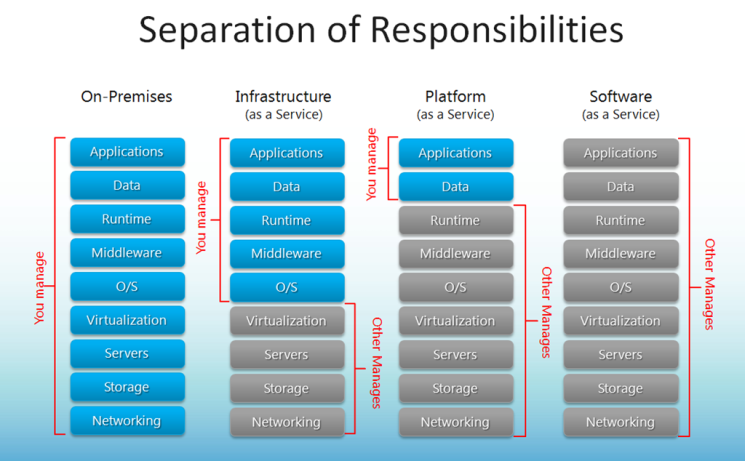
\includegraphics[width=0.8\textwidth]{chapters/background/images/separation-responsabilities.png}
	\caption[Separation of responsability in \acs{spi}]{Separation of responsability in different stacks
		of the \acf{spi} model compared with the on premises one \cite{spiRepsonabilities}.}
	\label{img:background-paas-spiResponsibilities}
\end{figure}

As we argued in Section \ref{sec:background-cloudComputing-cloudDepoymentModels}, \ac{paas} is possible
because is ``sitting'' over the \ac{iaas} infrastructure and through virtualization is able to provide many
features to developers. In following sections we will deep the concept of \ac{paas}
analysing its main characteristics and and the scenarios in which it is mostly useful and where it may not
be the best option. 

Later, in Section \ref{sec:background-virtualization} and \ref{sec:background-docker}, we will respectively
describe virtualization technique and containerization with Docker because they are used to ``build''
the software deployment units managed by the \ac{paas} level.

\subsection{Main characteristics}
\label{sec:background-paas-characteristics}
\ac{paas} offers to developers the following basic characteristics:

\begin{itemize}
	\item{it is able to maintain, inside the same \ac{ide}, services to develop, test and deploy
		applications;}
	\item{web based \ac{ui} creation tools help to create, modify, test and deploy different \ac{ui}
		scenarios;}
	\item{it makes possible multi-tenant architectures where multiple concurrent users utilize the same
		development application;}
	\begin{itemize}
		\item{support for development team collaboration: some \ac{paas} solutions can include project
			planning and communication tools;}
	\end{itemize}
	\item{it makes possible multi-tenant architectures where multiple concurrent users utilize the same
		deployed application\footnote{The application must be designed to support multiple concurrent
			users.};}
	\item{built in scalability of deployed software including load balancing and fault-tolerance;}
	\item{integration with databases and web services via common standards;}
	\item{tool to handle billing and subscription management.}
\end{itemize}

\ac{paas} is similar in many ways to \ac{iaas} but differentiate from it by the addition of value added
services and comes in two various types:

\begin{itemize}
	\item{a collaborative platform for software development, focused on workflow management regardless
		of the data source being used for the application. An example of this approach is Heroku, a
		\ac{paas} that utilizes Ruby on Rails language;}
	\item{a platform that allows for the creation of software that utilizing proprietary data from an
		application. This sort of \ac{paas} can be seen as a method to create applications with a common
		data form or type. An example is the Force.com from Salesforce.com which is used almost exclusively
		to develop applications that work with the Salesforce.com \ac{crm} tools.}
\end{itemize}

\ac{paas} owns the aforementioned characteristics because exploit better the feature that \ac{iaas}
is able to provide though virtualization. In the next section we will deep the concept of virtualization
to get to present the \acs{os} level of virtualization that cover a relevant part of this thesis.

\subsection{Where it makes sense}
\label{sec:background-paas-whereToUse}
\ac{paas} is very useful in any situation where multiple developers work on a development project or
where other external parties need to interact with the development process. As the case study illustrated
below, it is proving invaluable for those who have an existing data source, for example sales information
from a \ac{crm} tool, and want to create applications which leverage that data. Finally \ac{paas} is useful
where developers wish to automate testing and deployment services.

The popularity of \glossarySng{agile} will also increase the uptake of \ac{paas} as it eases the
difficulties around rapid development and iteration of software.

Some examples of \ac{paas} include \ac{gae} \cite{googleAppEngine}, Microsoft Windows Azure
\cite{windowsAzure} and finally Salesforce.com \cite{salesforcePlatform}.

\subsection{Where it may not be the best option}
\label{sec:background-paas-whereNotToUse}
There are many positive aspects that bring us adopting \ac{paas}, but there also some scenarios where it
may not be ideal. Examples include:

\begin{itemize}
	\item{where the applications need to be highly portable\footnote{In terms of where they are hosted.};}
	\item{where proprietary languages or approaches would impact on the development process;}
	\item{where a proprietary language would hinder later moves to others provides. Concerns are raised
		about vendor lock-in \cite{vendorLockin};}
	\item{where application performance requires customization of the underlying hardware and/or software.}
\end{itemize}

\subsection{A case study}
\label{sec:background-paas-caseStudy}
Menumate \cite{menumateCaseStudy} is a provider of point of sale hardware and software for the hospitality
industry across Australasia. It has taken advantage of the Force.com \ac{paas} to migrate over time a
series of legacy applications used in the business.

Trineo's \cite{trineoCaseStudy} directors of development explained that the use of Force.com platform has
allowed Menumate to centralise, modernise and integrate an otherwise disparate in-house software toolkit. 
They also asserted that a more conventional development approach would require significant infrastructure,
connectivity, security; this also would introduce uptime considerations. Instead the Force.com
platform inherently provides these non-functional requirements, allowing both Menumate and Trineo to
focus purely on developing the needed functionality. Additionally, utilizing a \ac{paas} approach
has meant Trineo could take advantage of both existing integration and deployment tools.

Utilizing a \ac{paas} development environment has resulted in the creation of applications being
significantly faster than would otherwise be the case. In absence of \ac{paas}, the cost of developing
applications would be prohibitive for many companies.